%%%%%%%%%%%%%%%%%%%%%%%%%%%%%%%%%%%%%%%%%
% Structured General Purpose Assignment
% LaTeX Template
%
% This template has been downloaded from:
% http://www.latextemplates.com
%
% Original author:
% Ted Pavlic (http://www.tedpavlic.com)
%
% Note:
% The \lipsum[#] commands throughout this template generate dummy text
% to fill the template out. These commands should all be removed when 
% writing assignment content.
%
%%%%%%%%%%%%%%%%%%%%%%%%%%%%%%%%%%%%%%%%%

%----------------------------------------------------------------------------------------
%	PACKAGES AND OTHER DOCUMENT CONFIGURATIONS
%----------------------------------------------------------------------------------------

\documentclass{article}

\usepackage{listings}
\usepackage{mathtools}
\usepackage{fancyhdr} % Required for custom headers
\usepackage{lastpage} % Required to determine the last page for the footer
\usepackage{extramarks} % Required for headers and footers
\usepackage{graphicx} % Required to insert images
\usepackage{lipsum} % Used for inserting dummy 'Lorem ipsum' text into the template
\usepackage{caption}
\usepackage{subcaption}
\usepackage{amsmath}

% Margins
\topmargin=-0.45in
\evensidemargin=0in
\oddsidemargin=0in
\textwidth=6.5in
\textheight=9.0in
\headsep=0.25in 

\linespread{1.1} % Line spacing

% Set up the header and footer
\pagestyle{fancy}
\lhead{\hmwkAuthorName} % Top left header
\chead{\hmwkClass} % Top center header   -->  \ (\hmwkClassInstructor\ \hmwkClassTime): \hmwkTitle
\rhead{\firstxmark} % Top right header
\lfoot{\lastxmark} % Bottom left footer
\cfoot{} % Bottom center footer
\rfoot{Page\ \thepage\ of\ \pageref{LastPage}} % Bottom right footer
\renewcommand\headrulewidth{0.4pt} % Size of the header rule
\renewcommand\footrulewidth{0.4pt} % Size of the footer rule

\setlength\parindent{0pt} % Removes all indentation from paragraphs

%----------------------------------------------------------------------------------------
%	DOCUMENT STRUCTURE COMMANDS
%	Skip this unless you know what you're doing
%----------------------------------------------------------------------------------------

% Header and footer for when a page split occurs within a problem environment
\newcommand{\enterProblemHeader}[1]{
\nobreak\extramarks{#1}{#1 continued on next page\ldots}\nobreak
\nobreak\extramarks{#1 (continued)}{#1 continued on next page\ldots}\nobreak
}

% Header and footer for when a page split occurs between problem environments
\newcommand{\exitProblemHeader}[1]{
\nobreak\extramarks{#1 (continued)}{#1 continued on next page\ldots}\nobreak
\nobreak\extramarks{#1}{}\nobreak
}

\setcounter{secnumdepth}{0} % Removes default section numbers
\newcounter{homeworkProblemCounter} % Creates a counter to keep track of the number of problems

\newcommand{\homeworkProblemName}{}
\newenvironment{homeworkProblem}[1][Problem \arabic{homeworkProblemCounter}]{ % Makes a new environment called homeworkProblem which takes 1 argument (custom name) but the default is "Problem #"
\stepcounter{homeworkProblemCounter} % Increase counter for number of problems
\renewcommand{\homeworkProblemName}{#1} % Assign \homeworkProblemName the name of the problem
\section{\homeworkProblemName} % Make a section in the document with the custom problem count
\enterProblemHeader{\homeworkProblemName} % Header and footer within the environment
}{
\exitProblemHeader{\homeworkProblemName} % Header and footer after the environment
}

\newcommand{\problemAnswer}[1]{ % Defines the problem answer command with the content as the only argument
\noindent\framebox[\columnwidth][c]{\begin{minipage}{0.98\columnwidth}#1\end{minipage}} % Makes the box around the problem answer and puts the content inside
}

\newcommand{\homeworkSectionName}{}
\newenvironment{homeworkSection}[1]{ % New environment for sections within homework problems, takes 1 argument - the name of the section
\renewcommand{\homeworkSectionName}{#1} % Assign \homeworkSectionName to the name of the section from the environment argument
\subsection{\homeworkSectionName} % Make a subsection with the custom name of the subsection
\enterProblemHeader{\homeworkProblemName\ [\homeworkSectionName]} % Header and footer within the environment
}{
\enterProblemHeader{\homeworkProblemName} % Header and footer after the environment
}
   
%----------------------------------------------------------------------------------------
%	NAME AND CLASS SECTION
%----------------------------------------------------------------------------------------

\newcommand{\hmwkTitle}{Project\ \#3} % Assignment title
\newcommand{\hmwkDueDate}{Tuesday,\ April\ 7,\ 2015} % Due date
\newcommand{\hmwkClass}{CSCI\ 8810} % Course/class
\newcommand{\hmwkClassTime}{08:00am} % Class/lecture time
\newcommand{\hmwkClassInstructor}{Prof. Arabnia} % Teacher/lecturer
\newcommand{\hmwkAuthorName}{Sina Solaimanpour} % Your name

%----------------------------------------------------------------------------------------
%	TITLE PAGE
%----------------------------------------------------------------------------------------

\title{
\vspace{2in}
\textmd{\textbf{\hmwkClass:\ \hmwkTitle}}\\
\normalsize\vspace{0.1in}\small{Due\ on\ \hmwkDueDate}\\
\vspace{0.1in}\large{\textit{\hmwkClassInstructor\ \hmwkClassTime}}
\vspace{3in}
}

\author{\textbf{\hmwkAuthorName}}
\date{} % Insert date here if you want it to appear below your name

%----------------------------------------------------------------------------------------

\begin{document}

\maketitle

%----------------------------------------------------------------------------------------
%	TABLE OF CONTENTS
%----------------------------------------------------------------------------------------

%\setcounter{tocdepth}{1} % Uncomment this line if you don't want subsections listed in the ToC

\newpage
\tableofcontents
\newpage

%----------------------------------------------------------------------------------------
%	Introduction
%----------------------------------------------------------------------------------------

% To have just one problem per page, simply put a \clearpage after each problem

\begin{homeworkProblem}[\Roman{homeworkProblemCounter}. Introduction]
In this paper, I will discuss about the third phase of the ColonD Image processing project. The first two phases of the project were about implementing some basic operations like read/write, gray-scale conversion, thresholding and smoothing images by applying filters and some of the most famous high-pass filters along with the CCL algorithm. In this phase of the of the project, I will expand the program to make it available to the user the feature to create an "N Level" pyramid out of an image and expand the pyramid levels to the size of the original image for further processing tasks. 


The following list shows what new features have been added to the program in phase 2:
\begin{itemize} \itemsep1pt \parskip0pt \parsep0pt
  \item Create an "N Level" Pyramid
  \item Expand the pyramid using Zero Order Hold Scheme
  \item Expand the pyramid using First Order Hold Scheme
\end{itemize}

These features are all implemented and tested with different images, individually and in combination of other operations. In the next sections, I will go over each one of these features in more detail and will present some results from the program.
\end{homeworkProblem}

%----------------------------------------------------------------------------------------
%	Pyramid
%----------------------------------------------------------------------------------------

% To have just one problem per page, simply put a \clearpage after each problem

\begin{homeworkProblem}[\Roman{homeworkProblemCounter}. Creating the Pyramid]

In order to create the pyramid, I go over each pixel of the original image and use the NS5 pixels to calculated the average intensity. After calculating this average, I will set the pixel in (i / 2, j / 2) in which i and j are the indexes for the current pixel in the original image. Other techniques could be used to down sample the image to create smaller size images, but when I tried this method, it turned out to be working fine. The resulting images from applying this technique to lena's image and the bike's image in shown in the previous reports can be shown in \textbf{Figure \ref{fig:lena_p}} and \textbf{Figure \ref{fig:bike_p}} respectively.

\begin{figure}[h!]
  \centering
	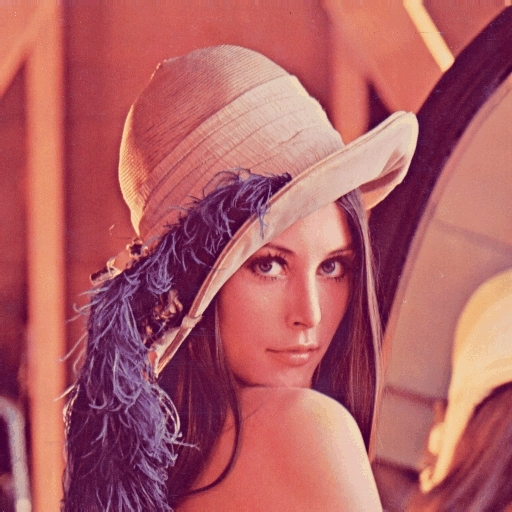
\includegraphics[width=0.3\textwidth]{Lena/p0}
	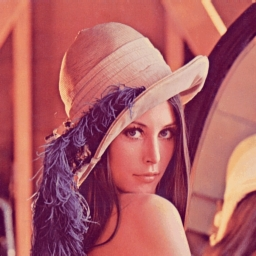
\includegraphics[width=0.15\textwidth]{Lena/p1}
	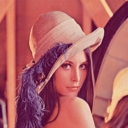
\includegraphics[width=0.075\textwidth]{Lena/p2}
	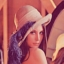
\includegraphics[width=0.0375\textwidth]{Lena/p3}
	
\includegraphics[width=0.01875\textwidth]{Lena/p4}
  \caption{The resulting pyramid from applying the pyramid creation algorithm to the Lena's picture. The images shown in this figure have relatively true sizes comparing to the first image on the left side.}
  \label{fig:lena_p}
\end{figure}

\begin{figure}[h!]
  \centering
	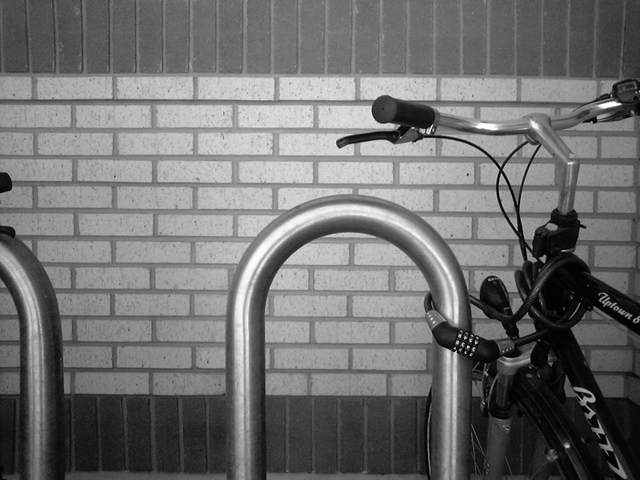
\includegraphics[width=0.3\textwidth]{Bike/p0}
	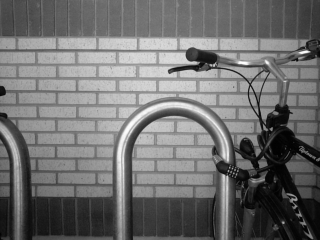
\includegraphics[width=0.15\textwidth]{Bike/p1}
	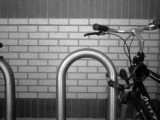
\includegraphics[width=0.075\textwidth]{Bike/p2}
	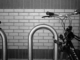
\includegraphics[width=0.0375\textwidth]{Bike/p3}
	
\includegraphics[width=0.01875\textwidth]{Bike/p4}
  \caption{The resulting pyramid from applying the pyramid creation algorithm to the Bike's picture. The images shown in this figure are in relatively true sizes comparing to the first image on the left side.}
  \label{fig:bike_p}
\end{figure}

Now, we need to resize the smaller images to be the same size as the original picture which are shown as the left most image in the figures. This will be done in the following sections using Zero order hold scheme and First order hold scheme techniques.

\end{homeworkProblem}

%----------------------------------------------------------------------------------------
%	Zero Order Hold Scheme
%----------------------------------------------------------------------------------------

% To have just one problem per page, simply put a \clearpage after each problem

\begin{homeworkProblem}[\Roman{homeworkProblemCounter}. Zero Order Hold Scheme]

This technique can be implemented by using a filter on an expanded image. This expanded image is twice the size of the original image and it has 0 as its pixel values every other rows or columns. This time, I preferred to implement this function without the help of my apply filter function just to see how it compares to its filter version. Instead, I used the algorithm discussed in class for zero order hold scheme without the use of filters. I create an image with twice the size of the original image and for each pixel, I create a 2 x 2 matrix in the result image. The resulting expanded images from the above pyramids using Zero order hold scheme are shown in \textbf{Figure \ref{fig:lena_o0}} and \textbf{Figure \ref{fig:bike_o0}}.

\begin{figure}[h!]
  \centering
	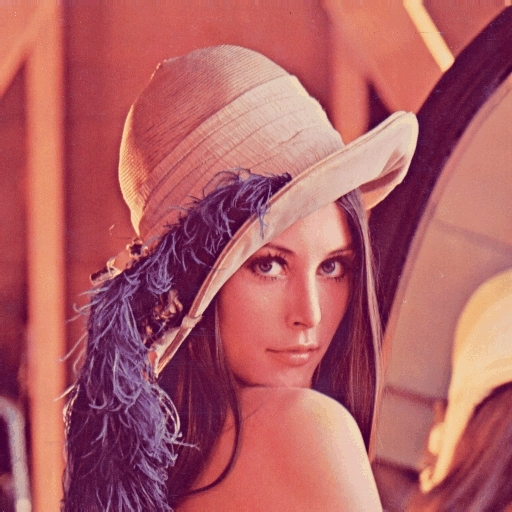
\includegraphics[width=0.3\textwidth]{Lena/o0l0}
	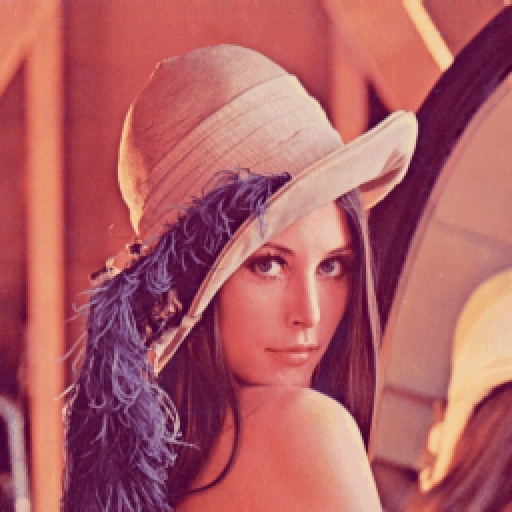
\includegraphics[width=0.3\textwidth]{Lena/o0l1}
	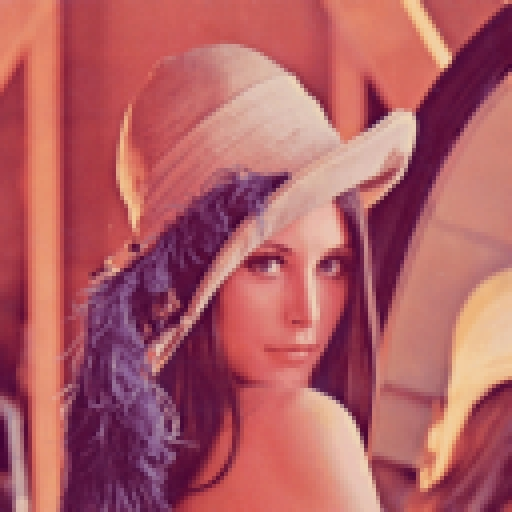
\includegraphics[width=0.3\textwidth]{Lena/o0l2}
	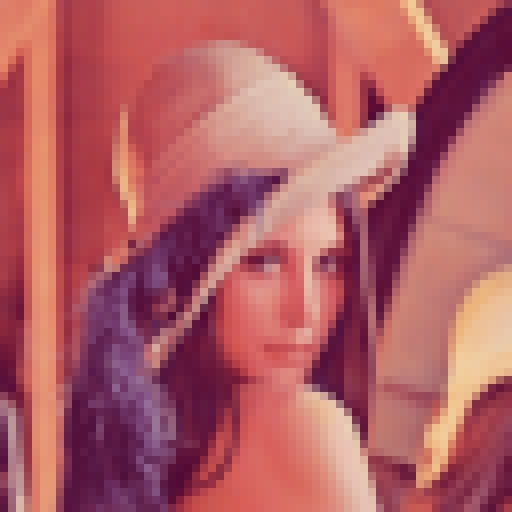
\includegraphics[width=0.3\textwidth]{Lena/o0l3}
	
\includegraphics[width=0.3\textwidth]{Lena/o0l4}
  \caption{Expanded images using Zero order hold scheme from the pyramid made out of the lena's image. The original image is shown as the top-left image and the lowest resolution image is shown as the bottom-right image.}
  \label{fig:lena_o0}
\end{figure}

\begin{figure}[h!]
  \centering
	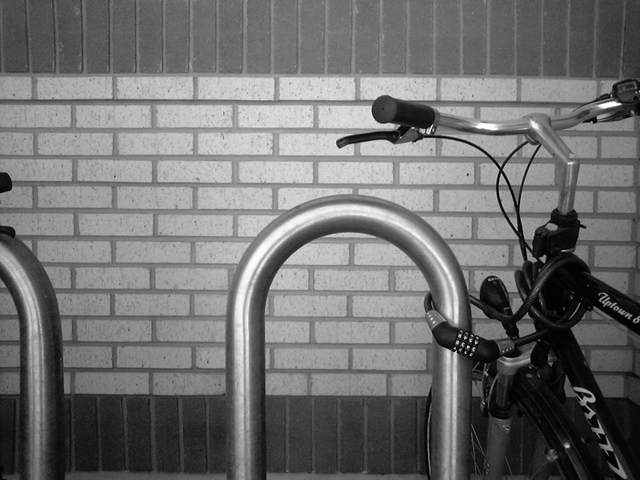
\includegraphics[width=0.3\textwidth]{Bike/o0l0}
	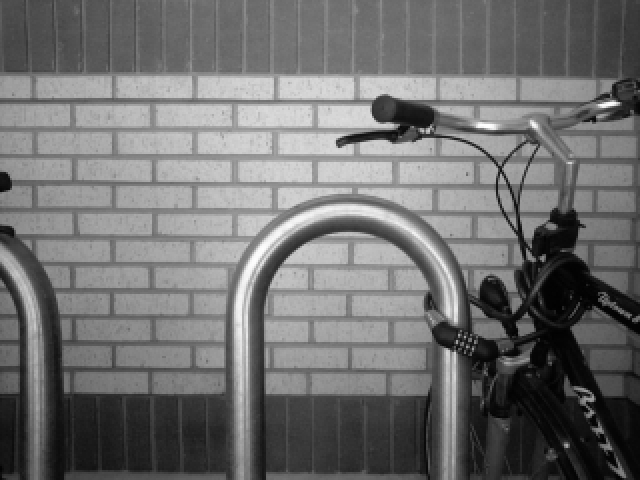
\includegraphics[width=0.3\textwidth]{Bike/o0l1}
	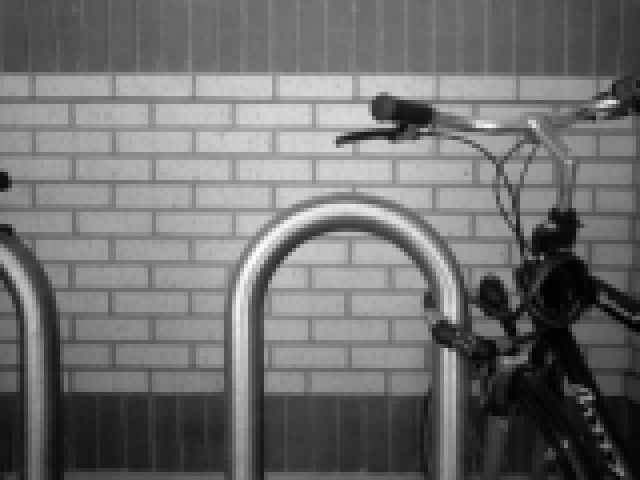
\includegraphics[width=0.3\textwidth]{Bike/o0l2}
	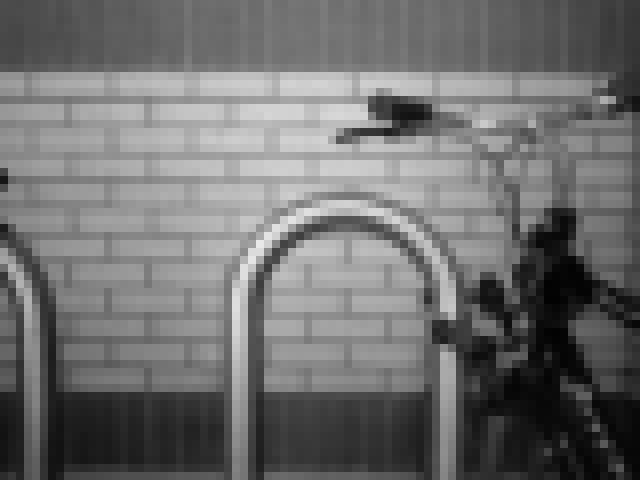
\includegraphics[width=0.3\textwidth]{Bike/o0l3}
	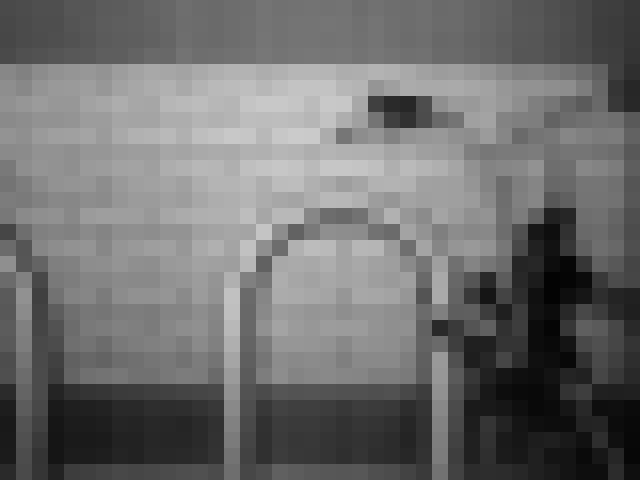
\includegraphics[width=0.3\textwidth]{Bike/o0l4}
  \caption{Expanded images using Zero order hold scheme from the pyramid made out of the bike's image. The original image is shown as the top-left image and the lowest resolution image is shown as the bottom-right image.}
  \label{fig:bike_o0}
\end{figure}

As it is visible in the images, when zero order hold scheme technique is applied multiple times to an image, it caused an box effect to appear in the resulting image. This boxing effect might be unpleasant when displaying the image but it also might be useful in other cases. In the following section, we will discuss about the First order hold scheme which will address this boxing effect issue.

\end{homeworkProblem}

%----------------------------------------------------------------------------------------
%	First Order Hold Scheme
%----------------------------------------------------------------------------------------

% To have just one problem per page, simply put a \clearpage after each problem

\begin{homeworkProblem}[\Roman{homeworkProblemCounter}. First Order Hold Scheme]

Unlike the zero order hold scheme technique, I implemented this one using the filter version algorithm. I expand the image just as described in the previous section and apply the filter introduced in class on the expanded image. 

\begin{figure}[h!]
  \centering
	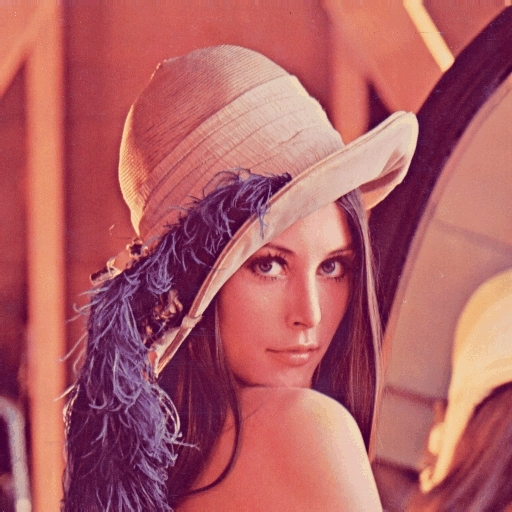
\includegraphics[width=0.3\textwidth]{Lena/o1l0}
	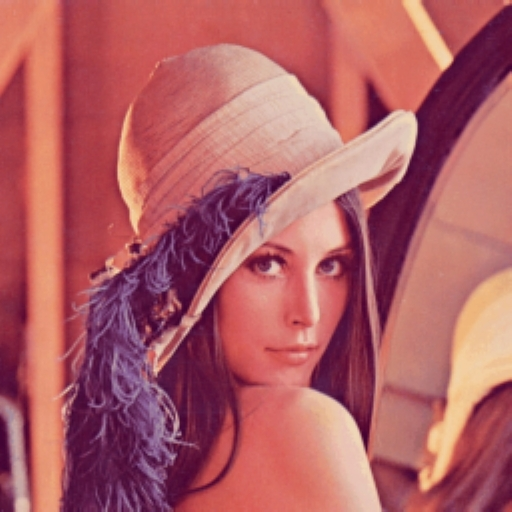
\includegraphics[width=0.3\textwidth]{Lena/o1l1}
	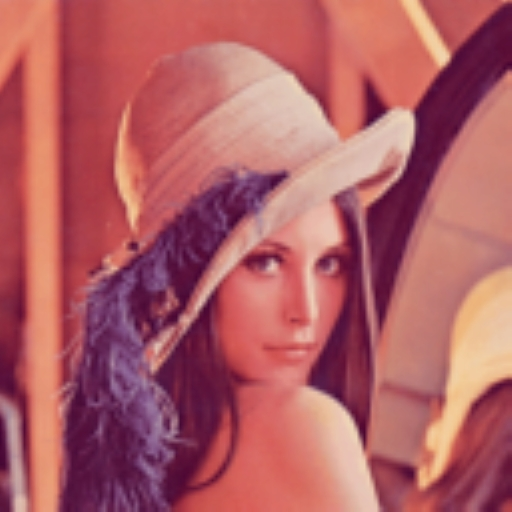
\includegraphics[width=0.3\textwidth]{Lena/o1l2}
	
\includegraphics[width=0.3\textwidth]{Lena/o1l3}
	
\includegraphics[width=0.3\textwidth]{Lena/o1l4}
  \caption{Expanded images using First order hold scheme from the pyramid made out of the lena's image. The original image is shown as the top-left image and the lowest resolution image is shown as the bottom-right image.}
  \label{fig:lena_o1}
\end{figure}

\begin{figure}[h!]
  \centering
	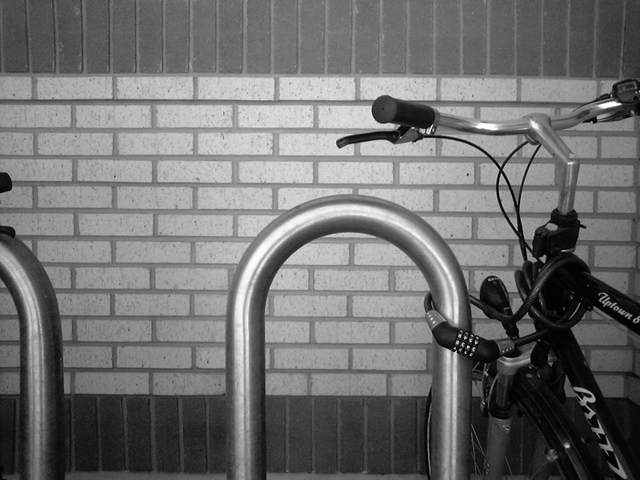
\includegraphics[width=0.3\textwidth]{Bike/o1l0}
	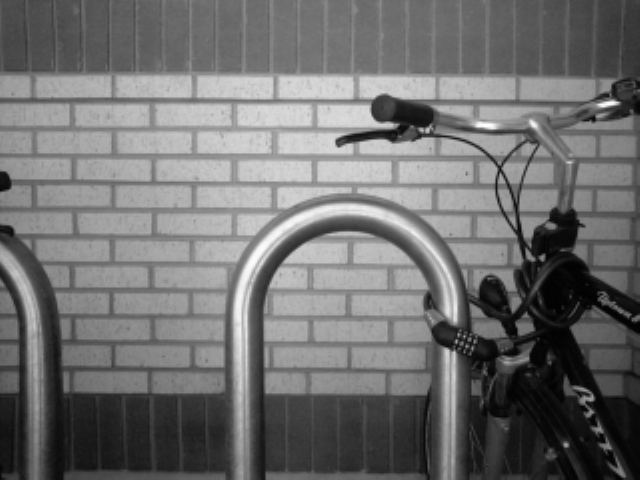
\includegraphics[width=0.3\textwidth]{Bike/o1l1}
	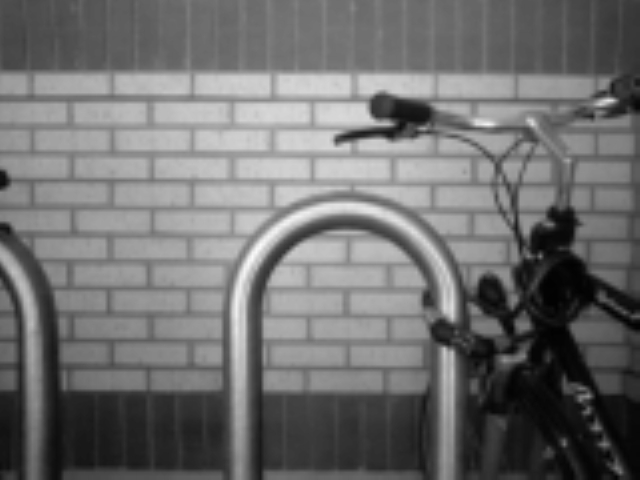
\includegraphics[width=0.3\textwidth]{Bike/o1l2}
	
\includegraphics[width=0.3\textwidth]{Bike/o1l3}
	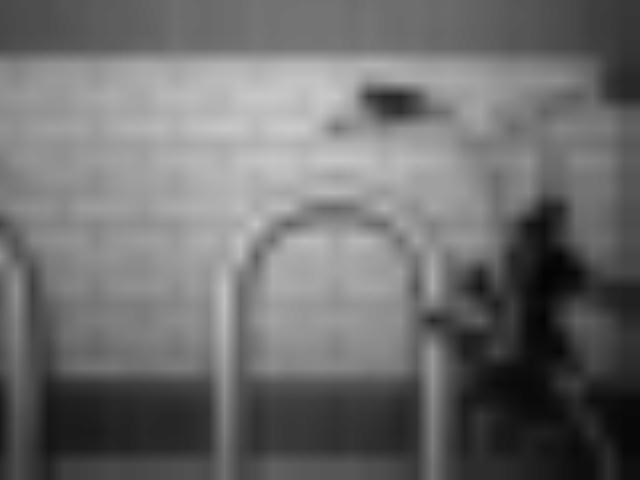
\includegraphics[width=0.3\textwidth]{Bike/o1l4}
  \caption{Expanded images using First order hold scheme from the pyramid made out of the bike's image. The original image is shown as the top-left image and the lowest resolution image is shown as the bottom-right image.}
  \label{fig:bike_o1}
\end{figure}

First order hold scheme technique, as depicted in \textbf{Figure \ref{fig:lena_o1}} and \textbf{Figure \ref{fig:bike_o1}}, will result in a much smoother expanded image in comparison with the Zero order hold scheme results. As it can be seen in the figures, the boxing effect is eliminated to some extend. This removal of the boxing effect is because of the use of interpolation between the pixel instead of just copying the same value four times. Using interpolation is because of the fact that pixel in true pictures change smoothly instead of jumping from one value to another in one step. 

\vspace{1cm}
\textit{In the following section, I try to show some interesting results from the experiments I had with the project.}

\end{homeworkProblem}

%----------------------------------------------------------------------------------------
%	Experiments
%----------------------------------------------------------------------------------------

% To have just one problem per page, simply put a \clearpage after each problem

\begin{homeworkProblem}[\Roman{homeworkProblemCounter}. Experiments]

In this section, I will show the results from the experiments that I did using the features implemented in this iteration of the project in combination of the features from the previous iterations. I used the pyramid in different combinations of different functions. The interesting result that saw was from the experiment which is described below,

\begin{enumerate} \itemsep1pt \parskip0pt \parsep0pt
	\item Create a 5 level pyramid out of the input image
	\item Expand the pyramid levels using the First order hold scheme technique
	\item Apply two 3 x 3 average smoothing to the image
	\item Apply Iterative Threshold to each level of the image
\end{enumerate}

The resulting images for both the lena and bike's pictures are shown in \textbf{Figure \ref{fig:lena_exp}} and \textbf{Figure \ref{fig:bike_exp}}.

\begin{figure}[h!]
  \centering
	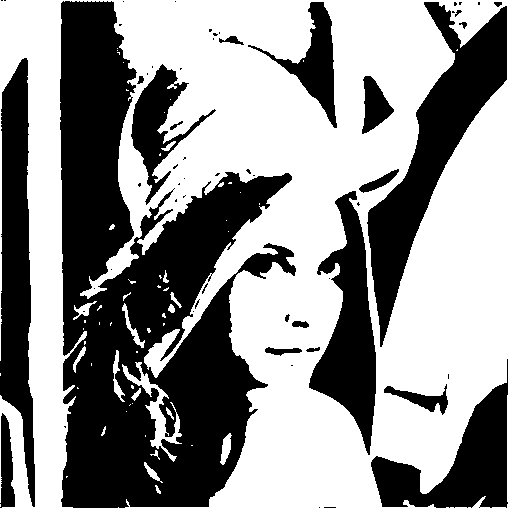
\includegraphics[width=0.3\textwidth]{Exp/ex0}
	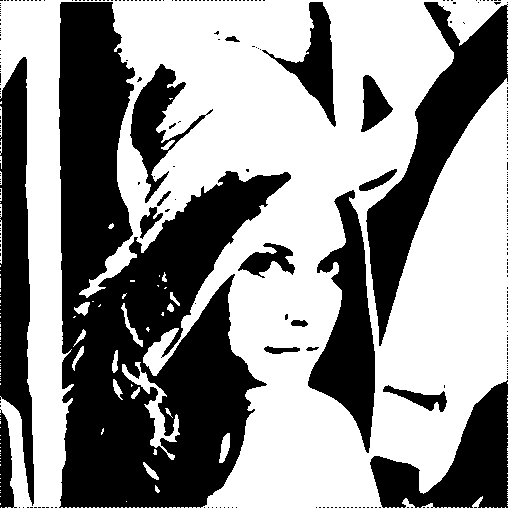
\includegraphics[width=0.3\textwidth]{Exp/ex1}
	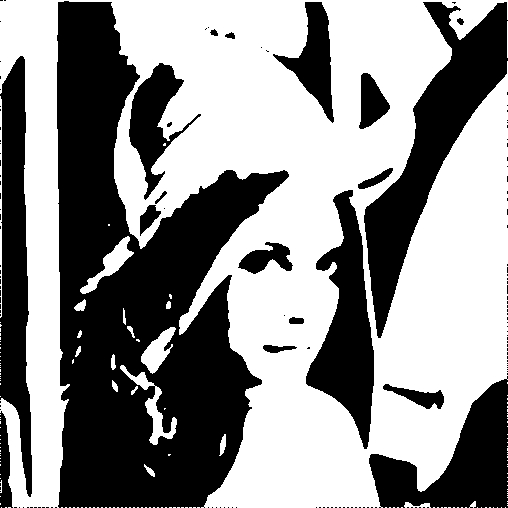
\includegraphics[width=0.3\textwidth]{Exp/ex2}
	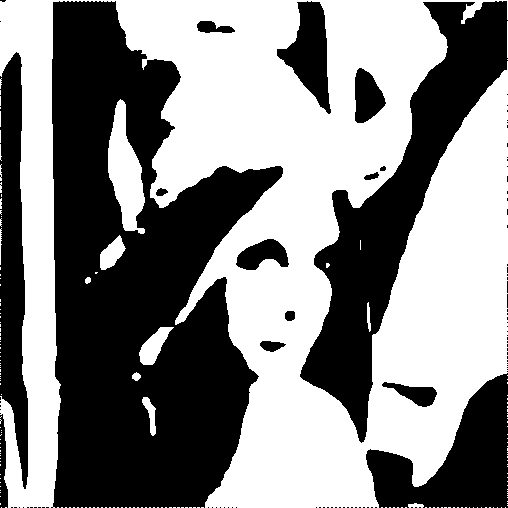
\includegraphics[width=0.3\textwidth]{Exp/ex3}
	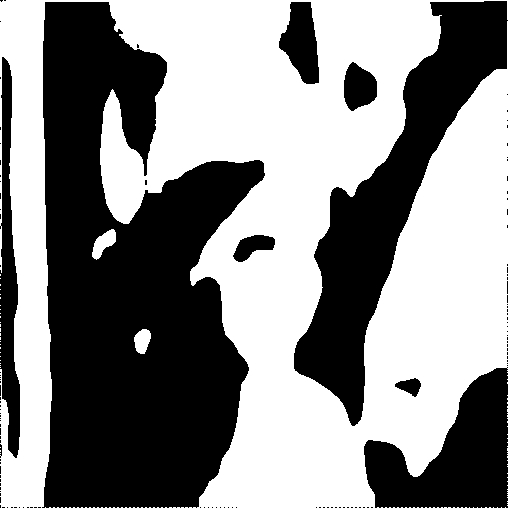
\includegraphics[width=0.3\textwidth]{Exp/ex4}
  \caption{Results from the experiment explained applied on the lena's picture.}
  \label{fig:lena_exp}
\end{figure}

\begin{figure}[h!]
  \centering
	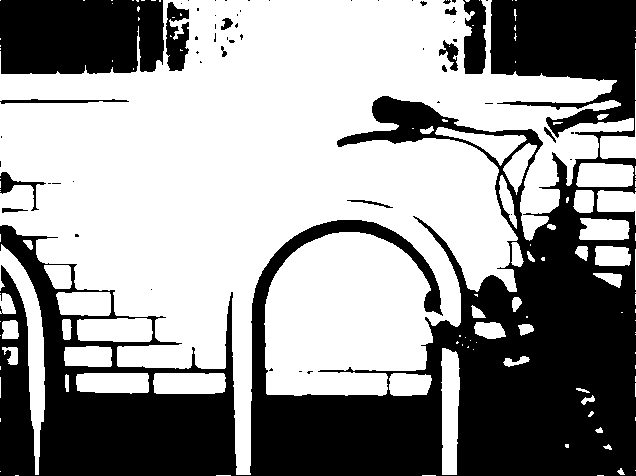
\includegraphics[width=0.3\textwidth]{Exp/bex0}
	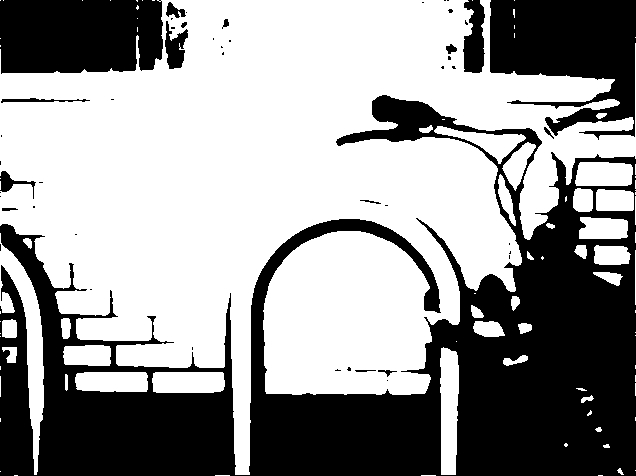
\includegraphics[width=0.3\textwidth]{Exp/bex1}
	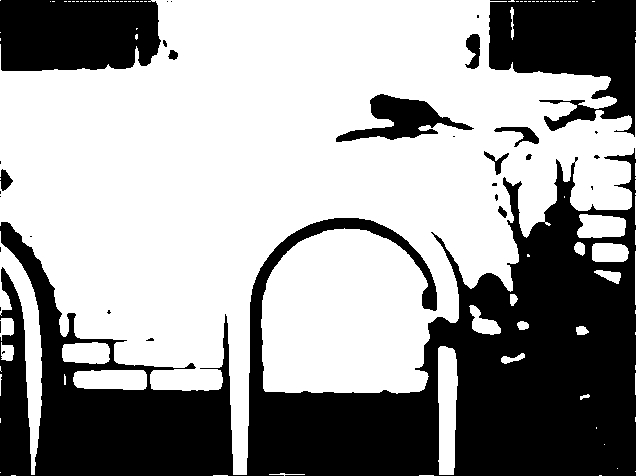
\includegraphics[width=0.3\textwidth]{Exp/bex2}
	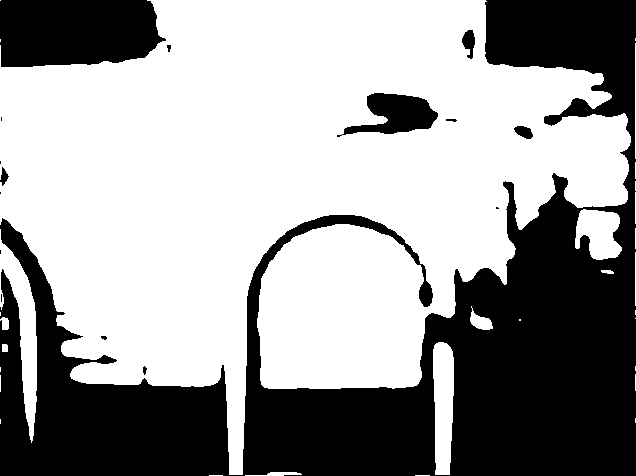
\includegraphics[width=0.3\textwidth]{Exp/bex3}
	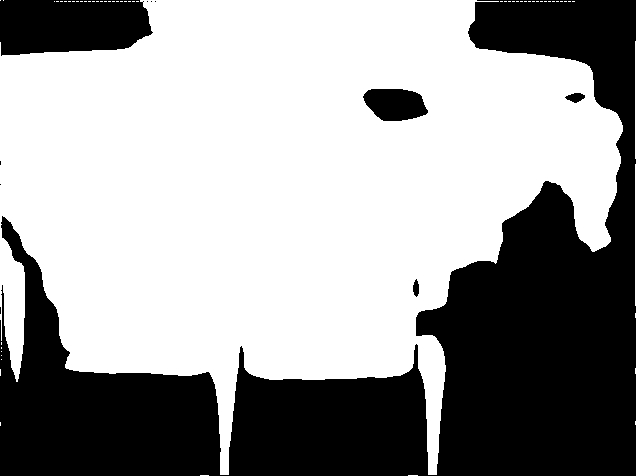
\includegraphics[width=0.3\textwidth]{Exp/bex4}
  \caption{Results from the experiment explained applied on the bike's picture.}
  \label{fig:bike_exp}
\end{figure}

As you can see, even though the images which are the result of the lower resolution images have less detail in them, they still have the overall structure of the image and the context can be understood even from looking at the binary version of the picture. For example, one can clearly see the picture of a woman in all level of the pyramid shown in Figure \ref{fig:lena_exp}. This tells us that there are valuable information that can help us process the image even in the lowest resolution image.

\end{homeworkProblem}


\end{document}
